\section{System design and composition}
\subsection{Model}
The system is modelled in two parts: the moving base and the\ldots
% TODO: describe the moving base, and the attachment, whatever it ends up being.
% Include physical models.


% Describe the states of the system.
We argue for the folloing five states of the system:
\begin{inline-enum}
\item waiting for a command;
\item moving to a destination;
\item following a navigation-line;
\item picking an object up; and
\item dropping an object off.
\end{inline-enum}
The relation between these five states are visually described in the state machine of Fig~\ref{fig:state_machine}.
\begin{figure*}[ht]
  \centering
  \begin{tikzpicture}
    \node[state, initial, accepting] (wait) {waiting for \\ command};
    \node[state, right of=wait] (move) {moving to \\ destination};
    \node[state, below of=move] (follow) {following \\ line};
    \node[state, right of=follow] (pickup) {picking \\ up object};
    \node[state, left of=follow] (dropoff) {dropping \\ off object};

    \path[->] (wait) edge node{Arrowhead \\ signal} (move)
    (move) edge[sloped] node{line detected \\} (follow)
    (follow) edge[sloped] node{station detection \\ (system w/o object)} (pickup)
    (follow) edge[sloped] node{station detection \\ (system w/ object)} (dropoff)
    (pickup) edge[sloped] node{object picked up \\} (move)
    (dropoff) edge[sloped] node{object dropped \\} (wait)
    ;
  \end{tikzpicture}
  \caption{High-level state machine of the system.}
  \label{fig:state_machine}
\end{figure*}
\subsubsection{Mobile platform}
The model used in this case is the unicycle model, due to the differential steering. 
This is because of the mobile platform has only two wheels/trucks and it is not able to apply any steering angle to its wheels. 
The only way this robot can change orientation is by giving different velocity on each wheel-driving servo on left- and right- side. 
With this feature it is also possible to change the orientation of the mobile platform without changing the position of the platform. 
I.e. the robot is able to spin while the right-hand sidewheels have the same velocity as the left-hand side wheels, in opposite direction. 

\begin{figure}[h!]
\centering
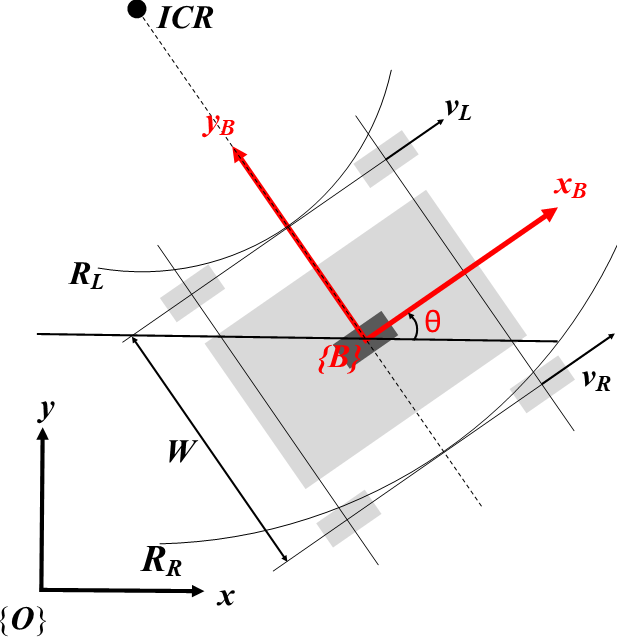
\includegraphics[width=0.4\textwidth]{sections/assets/car-unicycle.png}
\caption{Unicycle model of a car-like robot. 
$v_L$ and $v_R$ represent the left- and right-hand side wheels' velocities respectively. 
The robot follows a path around the instantaneous center of rotation (ICR) where $R_L$ and $R_R$ are the distances from left and right wheels to ICR respectively and $w$ is the distance between them.}
\label{fig:UnicycleModel}
\end{figure} 

As shown in Fig.~\ref{fig:UnicycleModel} The robot follows a curved path with the instantaneous center of rotation at its center. 
The left-hand side wheels have velocity $v_L$ and moves along an arc with radius $R_L$ during the time that right-hand side wheels moves along another arc with radius $R_R$ at the speed of $v_R$. 
The turning rate of the body is
        \begin{equation*}
            \dot{\theta}= \frac{v_L}{R_L} = \frac{v_R}{R_R}
        \end{equation*}
        since $R_R = R_L + W$ the expression can be simplified as
        \begin{equation}
            \dot{\theta}= \frac{v_R - v_L}{W} = \frac{v_\Delta}{W}\label{eq:ThetaDot3}
        \end{equation}
        the equations of motion for this model are
        \begin{eqnarray}
            \begin{aligned}
                \dot{x} &= v\,cos(\theta)\\
                \dot{y} &= v\,sin(\theta)\\
                \dot{\theta} &= \frac{v_\Delta}{W}
            \end{aligned}
            \label{eq:MotionEq3}
        \end{eqnarray}
        where the average velocity\parencite{Corke2011} is given by
        \begin{equation}
            v = \frac{v_R + v_L}{2} 
            \label{eq:av_velocity}
        \end{equation}{} 


\subsection{Simulation}
% Simulte the models from the previous section and show that it will work.
% Motivate regulation approach.

\subsection{Hardware}
% Explain the raspberry pi and it's attachments.

\subsection{Software}
\subsubsection{Reproducible system image generation}
% Explain the repo's *.nix files and what they do
The system image of the Raspberry Pi is generated via the repository's \texttt{mmc-image.nix} file ---
an auxiliary \texttt{build.sh} script is available to generate and subsequently flash a target storage device in a single command execution.
\texttt{mmc-image.nix} contains an expression of the Nix language.
Together with the usage of \texttt{nixpkgs} --- an extensive library of build and package declarations,
\texttt{mmc-image.nix} allows us to reliably and reproducibly build a bootable image of the complete software environment the project requires.
To then boot the generated image, it only needs to be flashed on a MultiMediaCard (MMC\footnote{Commonly referred to as: SD card, memory card.}) and slotted into the MMC-slot on the Raspberry Pi.

% Explain the pros of Nix
When building derivations (nomenclature for anything built with Nix: an executable binary, shared library file, a system environment, etc.) their dependencies are in complete isolation with each other, which effectively allows the avoidance of dependency hell.\footnote{Colloquial term referring to the frustration often generated when dealing with version-specific dependencies.
See \href{https://en.wikipedia.org/wiki/Dependency_hell}{Wikipedia}.}

% Explain the rollback functionality git provide us.
In combination with git, one may trivially roll back to previous derivations that are known to work by checking out a commit and rebuilding.

% Explain why treating the MMC as volatile is a good idea (MMCs have a tendency to just stop working).
In addition, by preferring a work flow where the target storage is considered volatile, any deficiencies of the target medium are mitigated.

% TODO: improve
\subsubsection{System-external services}
The software environment generated for the Raspberry Pi automatically connects to Eduroam if credentials are available.
Eduroam places some limitations on connected clients: firewall, e.g.
To enable easy remote access to the system, a reverse SSH proxy is established with a known bastion host which has a static IP address.
By exposing this proxy via a known port on the bastion, any system connected to the Internet may trivially access the Raspberry Pi remotely via a static endpoint.
While not a necessity for the project itself, this external service is a great convenience for ad-hoc experiments and general system debugging.

% Explain the content of contrib/bastion.nix
